%%%
%
% $Autor: Wings $
% $Datum: 2021-05-14 $
% $Pfad: LEDExternal $
% $Dateiname: 
% $Version: 4620 $
%
% !TeX spellcheck = de_DE/GB
% !TeX program = pdflatex
% !BIB program = biber/bibtex
% !TeX encoding = utf8
%
%%%

%todo citations
%todo create tikz pictures
%todo create sketches /ino-files with the code
%todo test the code

% Farben: https://rgbcolorcode.com/color/00FF00

\chapter{External Standard LED}


\section{General}

LED stands Light-Emitting Diode. A diode is an electronic component that only allows current to pass in one direction. Most diodes are made of semiconductor materials; in the case of light-emitting diodes, it is usually silicon.

The way an \ac{led} works is known from the animal world. For example, the energetic firefly is a flying \ac{led}. The only difference is how the atoms inside are excited and thus made to glow. The fireflies achieve this through a chemical reaction. In the \ac{led}, this happens with the help of an electric current - in short: electroluminescence.

A light-emitting diode consists of an anode (positive pole) and a cathode (negative pole). A wire, the so-called bonding wire, ensures the flow of current between the two poles. The energy required for electroluminescence flows through this wire. The semiconductor crystal (also known as the \ac{led} chip) sits on the cathode. It is surrounded by a reflector trough that directs the light from the \ac{led} chip upwards. The entire structure is embedded in a protective plastic lens. It distributes the light in the room, thereby increasing both the efficiency and the luminous efficacy.

The chip is a semiconductor crystal made from two different materials that are doped differently. Doping means that there is an excess of positive or negative charge carriers. When current flows, the electrons react and energy is released in the form of light flashes (photons). The \ac{led} lights up.

The color of the light depends on the doping of the semiconductor layers. Depending on the energy level, photons with different wavelengths, i.e. light color, are released. For example, a high energy level produces short-wave blue light and a low energy level produces long-wave red light. The superposition of the three primary colors red, blue and green produces white light. The colors red and green produce yellow. Red and blue become magenta, green and blue produce cyan.

A multicolor light-emitting diode therefore contains three semiconductor crystals, each of which produces one of the three primary colors and expands the color palette in different compositions.

Depending on how the brightness of red, green and blue is controlled, white is produced in different shades between very bright cool white light (indicated on the packaging as ``5000 Kelvin'' and above) or dimmed warm feel-good light (around 3000 Kelvin). As this variant of the mixture is expensive, there is now a new manufacturing option: blue \ac{led} chips are coated with a yellowish phosphor layer.

The colors available for ac{led}s are quite diverse, ranging from the basic red, green, and blue (RGB) to a much wider spectrum depending on the technology and application. \cite{Quadrios:2020} Here's a breakdown of the different types:

\begin{description}
  \item[Red:] This is the most common LED color, achieved by using materials like gallium arsenide phosphide (GaAsP). It has a dominant wavelength around 620-750 nm and appears vibrant red to the human eye.
  \item [Green:] Another common LED color, typically made with indium gallium nitride (InGaN). Its dominant wavelength falls between 500-570 nm, producing a bright green color.
  \item [Blue:] Blue LEDs are often made with gallium nitride (GaN) and emit light with a dominant wavelength of 450-480 nm. They appear as a deep, rich blue to our eyes.
\end{description}  

\medskip
  
Combinations and White Light:

\begin{description}
   \item [White:] While not a single color, white LEDs are crucial for various applications. They are typically achieved in two ways:
     \begin{itemize}
       \item RGB combination: Combining red, green, and blue LEDs in specific ratios can create white light. This method offers flexibility in color temperature control.
       \item Phosphor conversion: A blue or ultraviolet LED is coated with a phosphor that converts part of the emitted light to longer wavelengths, generating white light. This method is more efficient but offers less color control.
     \end{itemize}
\end{description}

\medskip


Beyond the Basics:

\begin{description}
  \item [Amber:] Often used in traffic signals and indicator lights, amber LEDs have a dominant wavelength around 585-605 nm and appear yellowish-orange.
  \item [Yellow:] True yellow LEDs are less common but achievable with specific materials like aluminum gallium indium phosphide (AlGaInP). Their dominant wavelength is around 580-590 nm, appearing as a pure yellow color.
  \item [Other colors:] Specialized LEDs can produce various other colors, including violet, pink, cyan, and even deep red and green for wider spectrum applications. These often involve more complex materials and manufacturing processes.
\end{description}

It's important to note that the specific color of an ac{led} can vary slightly depending on factors like manufacturing tolerances, viewing angle, and operating conditions. Additionally, new ac{led} technologies are emerging constantly, potentially expanding the color range further in the future.
\cite{Kainka:2009, Hering:2021,Hering:2023,Baichtal:2018}




\section{Specification}    


A \ac{led} need to have a resistor placed in series with it. Otherwise, the unrestricted current will quickly burn out the \ac{led}. The resistor can be any value between 100 Ohms and about 10K Ohms. It is necessary to check the data sheet. Lower value resistors will allow more current to flow, which makes the \ac{led} brighter. Higher value resistors will restrict the current flow, which makes the \ac{led} dimmer. A typically value is 220 Ohm. Using the data sheet of the LED, the value of the resistor can be determined. \cite{Quadrios:2020,Huiyuan:2017}
The maximal current to operate an \ac{led} is 20mA. It works also using 4mA until 15 mA. \cite{Quadrios:2020}


Most \ac{led}s have polarity, which means that they need to be connected the right way around. Usually, the \ac{led}'s shortest lead connects to the ground side, see figure \ref{LED:Standard}

\begin{center}
%todo tikz picture with strip red - red - black - brown 1\%
% or red - red - black - gold 5\%

\includegraphics[width=0.8\textwidth]{Sensor/Resistor/R}
  \captionof{figure}{Resistor with 220 Ohm for an external LED.}
\end{center}


%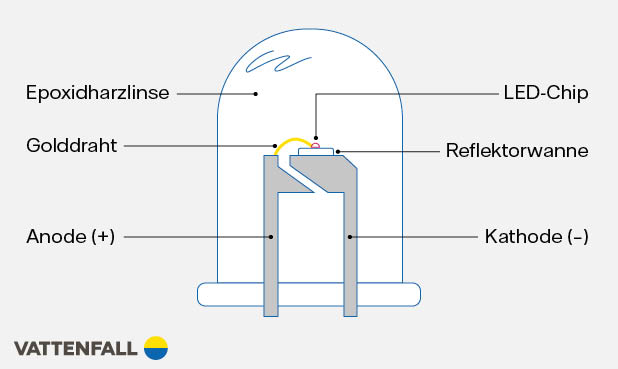
\includegraphics[width=0.8\textwidth]{Sensor/LED/LEDDesign.jpg}

\begin{center}
%todo tikz picture  
  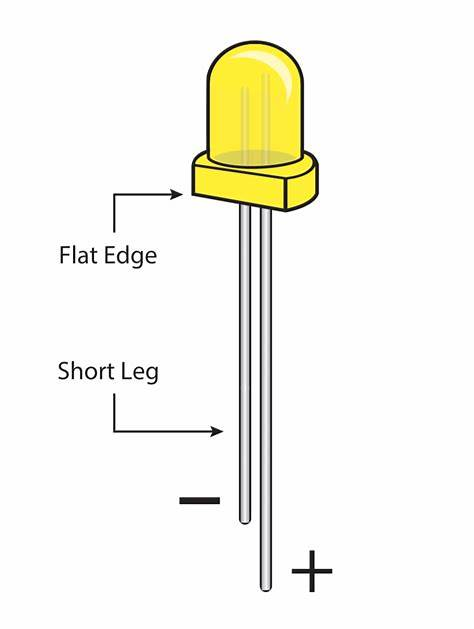
\includegraphics[width=0.3\textwidth]{Sensor/LED/LED.jpg}\quad
  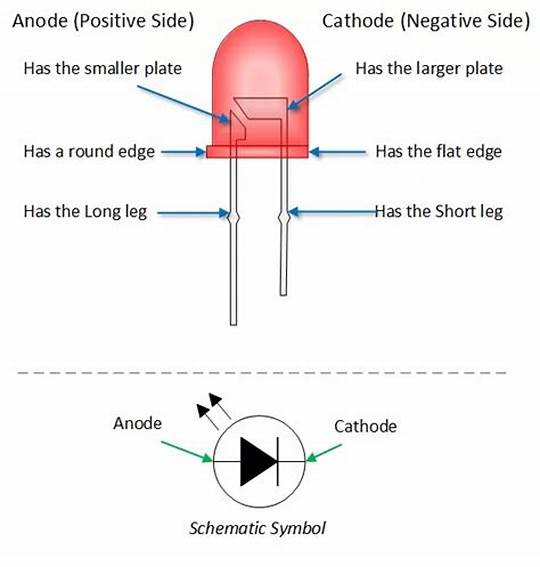
\includegraphics[width=0.3\textwidth]{Sensor/LED/LED2.jpg}
  \captionof{figure}{Parts of a LED.}\label{LED:Standard}
\end{center}

\begin{center}
%todo tikz picture  
  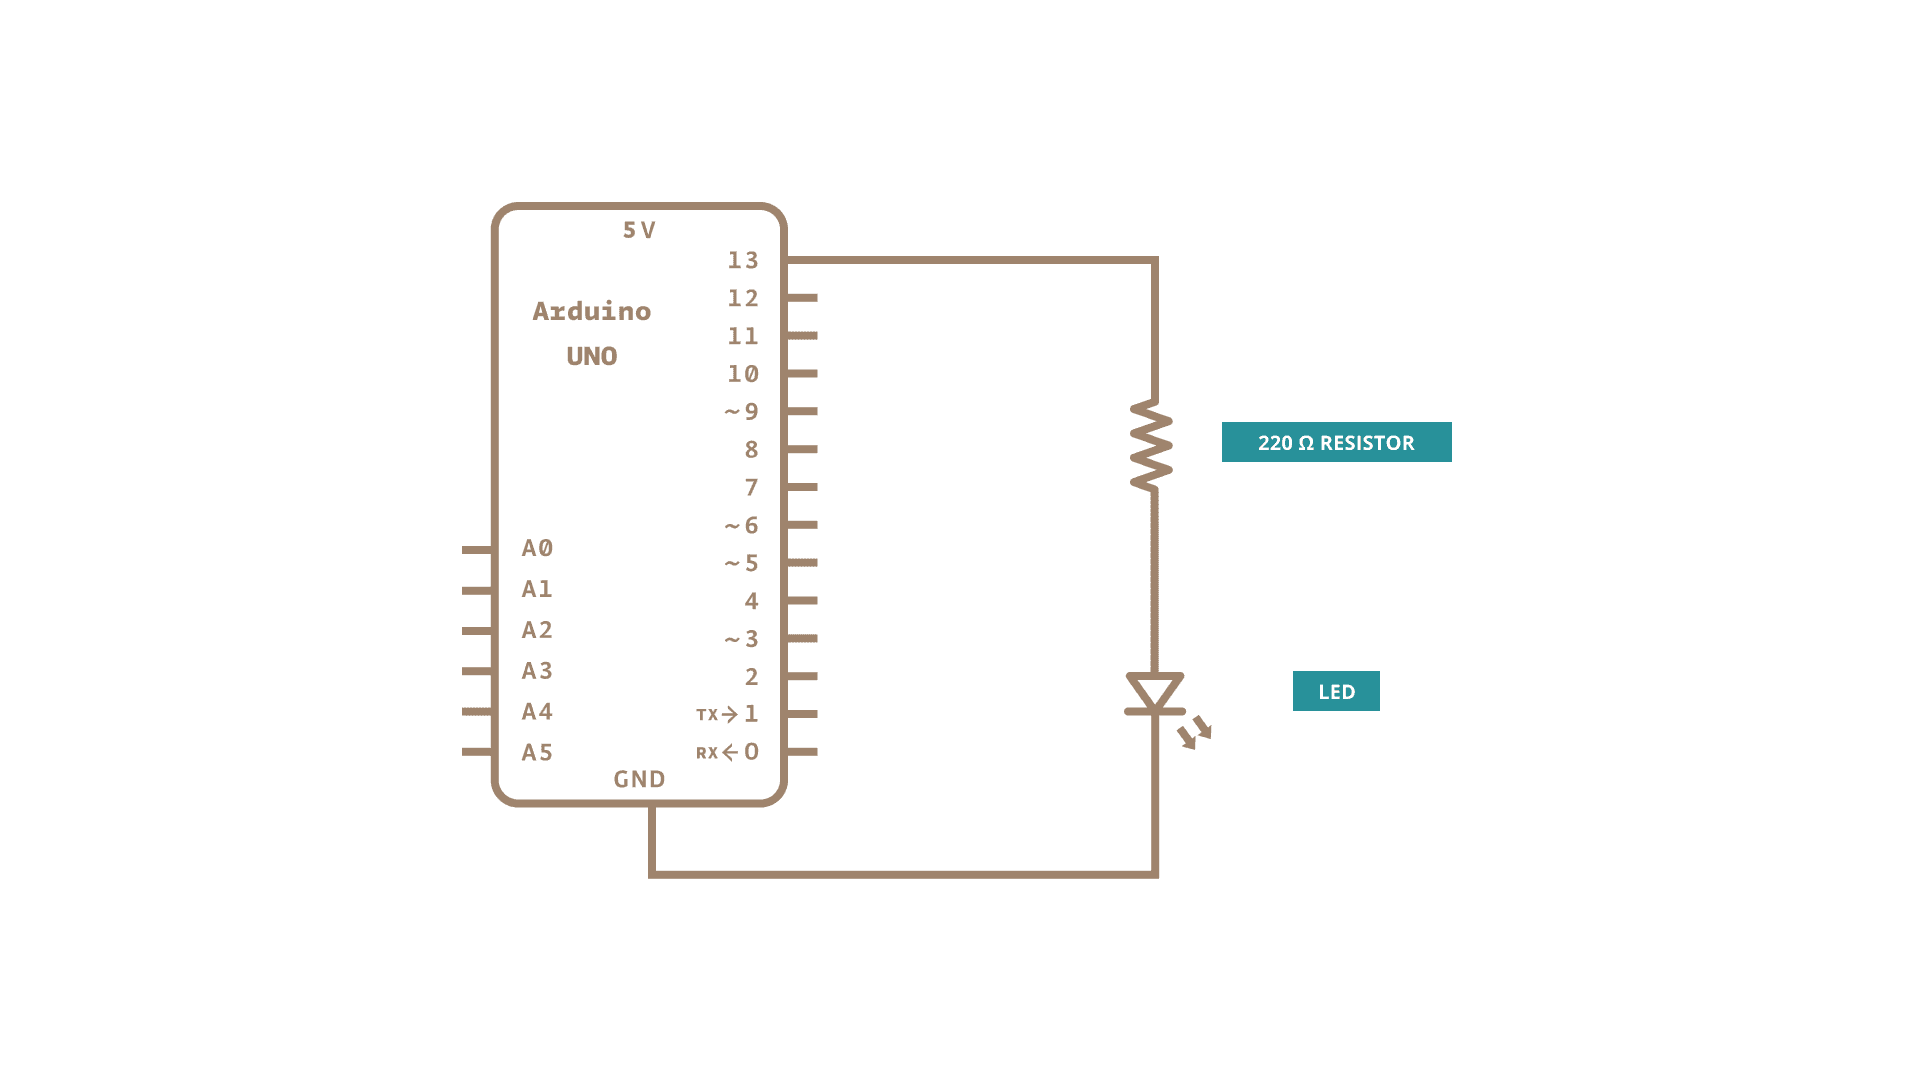
\includegraphics[width=0.8\textwidth]{Sensor/LED/circuitLED}
  \captionof{figure}{Schematic Symbol for a LED.}

\end{center}  


The Arduino can control as many \ac{led}s as long as there are enough pins available. 



\section{Using Standard External LED}\index{LED!Standard LED}


\subsection{Connecting a LED to the Arduino Board}

\Mynote{create  a diagram that shows how to connect a common cathode RGB LED to the board}


\subsection{Pins}

As mentioned, the Arduino can control as many \ac{led}s as long as there are enough pins available. There two different types of output pins
The standard output pin can just switch between high and low. For some pins the \ac{pwm} is usable. Usiing such a pin, the brightness of the ac{led} can be controlled.

\Mynote{Which pins}

PWM  A0 - A7 Welche Nummer? 16-23? 19 - 26

Digital D2-D13 Welche Nummer Pin 5 -16


\Mynote{Grafik!}


\section{Bibliothek}

No special library is required to operate an external LED.



\section{Simple Code}


As soon as the ac{led} is connected, it can be used. It is not necessary to install a special library.
Programming takes place in three steps:

\begin{enumerate}
    \item In the first step, the ac{led} must be connected to a pin:
    
    {
        \captionof{code}{Defining the pin for an external LED}
        \begin{Arduino}
            #define LED_EXT 14
        \end{Arduino}
    }
    \item In the second step, the pin is configured in the function \PYTHON{setup}:
    
    {
        \captionof{code}{Defining the pin for an external LED}
        \begin{Arduino}
            pinMode(LED_EXT, OUTOUT)   
        \end{Arduino}
    }
    \item In the third step, the ac{led} can be used in the function \PYTHON{loop}. To turn OFF the \ac{led}s, write a state \PYTHON{LOW} to the \ac{led}:
    
    {
        \captionof{code}{Swichting On the LED}
        \begin{Arduino}
            // Swichting On the LED        
            digitalWrite(LED, HIGH); 
            //Waiting 1s
            delay(1000)
            // Swichting Off the LED
            digitalWrite(LED, LOW);
        \end{Arduino}
    }
    
\end{enumerate}



\section{Tests}

\subsection{Simple Function Test}

The simplest test is the flashing of the LED at 2 Hz, see sketch \ref{Nano:LEDTest}.

{
    \captionof{code}{Simple sketch to test a LED}\label{Nano:LEDTest}
    \ArduinoExternal{}{../../Code/Nano33BLESense/Test/TestLED.ino}
}



\subsection{Test all Functions}

Standard pins can be used, but pins that support pulse width modulation can also be used. One such pin is used in the example \ref{Nano:TestLEDPWM}. The brightness can then be varied.

{
    \captionof{code}{Simple sketch to test a LED with pulse width modulation}\label{Nano:TestLEDPWM}
    \ArduinoExternal{}{../../Code/Nano33BLESense/Test/TestLEDBrightness.ino}
}



%%%%%%%%%%%%%%%%%%%%%%%%%%%%%%%%%%%%%

\section{Simple Application}

In the sketch \ref{Nano:TestLEDInterrupt}, a variable is connected to pin 14.\index{Pin!Pin 14} The pin is defined as an output in the function \PYTHON{setup}.
An interrupt function is defined, changing the state of a flag. If the flag has the value \PYTHON{true}, the led is switch on for 2 seconds. After the 2 seconds, the led is switch off and the value of the flag is set to \PYTHON{false} back.


{
    \captionof{code}{Simple sketch to control an external  LED. Here, pushing the built-in button is handled by an interrupt. Then the LED switch on for 2 sec.}\label{Nano:TestLEDInterrupt}
    \ArduinoExternal{}{../../Code/Nano33BLESense/Test/TestPushButtonInterrupt.ino}
}

\bigskip

This is just a simple example. The variable \PYTHON{BUTTON\_B} is already defined, so the assignment is not necessary. The command \PYTHON{delay} should be avoided in an Arduino sketch. Instead, variables of the type \PYTHON{elapsedMillis} should be used.


\section{Further Readings}


\Mynote{citations}









